% ==============================================================================
% T0 Theory / FFGFT: Document 285 (Chapter Content, EN)
% Title: The unified compactified picture (T^N, G) and the computed 3-vs-6 bridge
% Author: Johann Pascher
% Date: 19 June 2026
% References: Doc. 206, 230, 248, 249, 270, 281, 282, 283.
% Scripts: dim_bridge_1_doubling.py, dim_bridge_2_crystallographic.py,
%          dim_bridge_3_same_ambient_fork.py
% ==============================================================================

\section*{Abstract}
FFGFT and HLV both reduce to the observable $3{+}1$. This raises a sharp question: if
the four circles of FFGFT and the six (plus time) of HLV both end in $\mathbb{R}^3\times
\mathbb{R}_t$, are the $3$ and the $6$ merely two coordinate descriptions of the same
thing -- i.e.\ only a mathematical transformation? This document gives the compact-view
answer in one notation and checks it by computation. In the compact picture both models
are of the same form: a torus $T^N=(S^1)^N$ carrying a finite symmetry group $G$, with a
Type-I decompactification (the measurement) selecting one circle as time. FFGFT is
$(T^4, \mathbb{Z}_3)$; HLV is $(T^7=T^6\times S^1, A_5)$. Three reproducible results
settle the question. (1)~``$6$ is the doubling of the $3$'' is literal: the icosahedral
$6$D representation splits as $\mathbf{3}\oplus\mathbf{3'}$, the two $3$D irreducibles of
$A_5$, differing exactly by $\varphi\leftrightarrow 1-\varphi$; the $6$D character is an
integer while each $3$D block is irrational ($\varphi$). (2)~The triangle is the more
fundamental, minimal carrier: $3$-fold symmetry is crystallographic and lives in $3$D,
while $5$-fold is non-crystallographic and \emph{requires} the $6$D embedding. (3)~The two
models are \emph{reconcilable by containment}: the icosahedral group $A_5$ contains the
$3$-fold $C_3$ (both are symmetries of the same icosahedron), and $T^7=T^4\times T^3$, so
HLV is FFGFT's $4$D extended by the three perp dimensions ($7=4+3$, $\mathrm{HLV}\supset
\mathrm{FFGFT}$). The protected values $\sqrt2$ (Koide $2/3$) and $2/\sqrt5$ ($\varphi$) belong to two
\emph{different protected geometries} -- FFGFT's independent $3$-fold and HLV's $5$-fold;
the groups coexist ($C_3<A_5$), so this is no incompatibility, and the cut-and-project
family $r(\tau)\le1$ failing to map one onto the other shows only that interconversion is
the wrong question. (Per Doc.~283, $\sqrt2$ is \emph{not} inherited from HLV's
icosahedrally protected directions, which give only $2/\sqrt5$; it is a separate $3$-fold
protected choice.) The genuine difference is \emph{which symmetry sector is physically
realised}: FFGFT realises the minimal crystallographic $3$-fold core (Koide $\theta=2/9$,
empirically confirmed), while HLV adds the $5$-fold/perp structure as a testable extension.
Hence ``only a mathematical transformation'' is too weak (the realised sector is a genuine,
empirically decidable feature) and ``inequivalent structures'' is too strong (they are
reconcilable, $\mathrm{HLV}\supset\mathrm{FFGFT}$): the precise statement is a shared
$3{+}1$ core with HLV the icosahedral extension of FFGFT's minimal $3$-fold core.

% ==============================================================================
\section{Occasion: both reduce to $3{+}1$ -- is the rest a transformation?}
% ==============================================================================
Doc.~270 separates the reductions of FFGFT ($T^4\to 3{+}1$) and Doc.~283 the
FFGFT$\leftrightarrow$HLV relation (a $\mathbb{Z}_3$-circulant bridge along a $C_3$ axis,
forked at the symmetry order, $\sqrt2$ vs $2/\sqrt5$). HLV builds space as a $6$D$\to3$D
icosahedral cut-and-project and carries time separately (spiral-time). Both models
therefore end in the same observable $\mathbb{R}^3\times\mathbb{R}_t$. The natural
question is whether the difference between FFGFT's $3$ and HLV's $6$ is then merely a
choice of coordinates -- a lossless mathematical transformation of one and the same
$3{+}1$. The answer requires a common notation and a computation; both are given here. All
numerical statements are reproducible with three short scripts (\S\ref{sec:repro}).

% ==============================================================================
\section{The unified compactified notation $(T^N, G)$}
% ==============================================================================
In the compact representation there is no ``space'' versus ``time'' and no
``internal'' versus ``external'': a circle is a circle. Both models are then of one form:
\begin{equation}
\mathcal{M}=T^N=(S^1)^N,\qquad G\subset O(N)\ \text{acting,}
\end{equation}
with a Type-I decompactification (the measurement) selecting one circle as time. The
remaining circles stay compact (discrete spectrum) or project (space, Type~II,
Doc.~270). The two models are two instances of $(T^N,G)$:

\begin{center}\small
\renewcommand{\arraystretch}{1.3}
\begin{tabular}{@{}p{3.5cm} p{4.4cm} p{4.7cm}@{}}
\toprule
 & \textbf{FFGFT} & \textbf{HLV} \\
\midrule
compact form & $T^4=(S^1)^4$ & $T^7=T^6\times S^1$ \\
symmetry group $G$ & $\mathbb{Z}_3$ (3-fold, crystallographic) & $A_5$ icosahedral (5-fold, non-crystallographic) \\
space (compact) & $3$ circles & $6$ circles $=\mathbf{3}\oplus\mathbf{3'}$ \\
time & one circle (mass circle, $\tilde{T}\cdot m=1$); scale-linked by the duality, \emph{not} a split-off factor & one circle (spiral-time); an $A_5$-singlet, so the torus \emph{factorises} $T^6\times S^1$ \\
how $G$ acts on time & woven in through $\tilde{T}\cdot m=1$ & trivially (singlet) \\
protected invariant & $r=\sqrt2$, Koide $Q=2/3$, $\theta=2/9$ & $r=2/\sqrt5$, $\varphi$ \\
why this $N_\text{space}$ & $3$ suffices ($3$-fold crystallographic) & $6$ needed ($5$-fold non-crystallographic) \\
\bottomrule
\end{tabular}
\end{center}

The whole comparison reduces to one question -- \emph{how does $G$ act on the circles of
the torus?} The labels ``internal/external'' are decompactification language and have no
place in the compact picture; the correct compact-view distinction for the time circle is
group-theoretic: in HLV it is an $A_5$-singlet (the torus factorises $T^6\times S^1$,
time decoupled from the spatial symmetry); in FFGFT it is tied to the other circles by the
duality $\tilde{T}\cdot m=1$ (not a direct-product factor). Which circle becomes the
observed time is fixed by the measurement, i.e.\ the experienced situation of the embedded
observer (Doc.~270, Doc.~248), not by the geometry.

% ==============================================================================
\section{``$6$ is the doubling of the $3$'' -- literal (\texttt{dim\_bridge\_1})}
% ==============================================================================
The icosahedral $6$D representation used in the cut-and-project decomposes as
\begin{equation}
\mathbf{6} \;=\; \mathbf{3}\oplus\mathbf{3'},
\end{equation}
the two inequivalent $3$D irreducible representations of $A_5$ (physical $\oplus$ perp).
On the $5$-fold conjugacy class the characters are
\begin{equation}
\chi_{\mathbf 3}(g_5)=1+2\cos 72^\circ=\varphi,\qquad
\chi_{\mathbf 3'}(g_5)=1+2\cos144^\circ=1-\varphi=-\tfrac1\varphi,\qquad
\chi_{\mathbf 6}(g_5)=1.
\end{equation}
So the doubling is literal -- $\mathbf 6$ is two copies of a $3$D space -- and the golden
ratio sits \emph{in the split itself}: the two $3$D blocks differ exactly by
$\varphi\leftrightarrow 1-\varphi$. The $6$D character is the integer $1$ while each $3$D
block is irrational ($\varphi$); this is the first half of why a $6$D lattice exists where
a $3$D one cannot (next section). This $\varphi$ in the doubling is HLV's $5$-fold /
$2/\sqrt5$ at its root (cf.\ Doc.~281, Doc.~283).

% ==============================================================================
\section{The triangle is fundamental, the pentagon needs the six (\texttt{dim\_bridge\_2})}
% ==============================================================================
A rotation of order $n$ is a lattice symmetry in $2$D/$3$D if and only if
$2\cos(2\pi/n)\in\mathbb{Z}$ (crystallographic restriction). The integer values occur only
for $n\in\{1,2,3,4,6\}$:
\begin{equation}
2\cos\tfrac{2\pi}{3}=-1\in\mathbb{Z}\quad(\text{3-fold, crystallographic}),\qquad
2\cos\tfrac{2\pi}{5}=\tfrac1\varphi\notin\mathbb{Z}\quad(\text{5-fold, forbidden}).
\end{equation}
Hence $3$-fold symmetry ($\mathbb{Z}_3$, Koide) lives natively in $3$D -- three dimensions
\emph{suffice}, and the triangle is the minimal, more fundamental carrier. $5$-fold
symmetry cannot sit in a $3$D lattice; it exists only as a projection from $6$D, where (by
the previous section) it acquires an integer character. The doubling $3\to6$ is therefore
not optional decoration: it is exactly what hosting a non-crystallographic symmetry costs.

% ==============================================================================
\section{Same ambient $3{+}1$: what the cut-and-project family does and does not show (\texttt{dim\_bridge\_3})}
% ==============================================================================
The cut-and-project ratio
\begin{equation}
r(\tau)=\frac{2\tau}{1+\tau^2}\le 1,\qquad r(1)=1,
\end{equation}
is the family of cut-and-project ``mathematical transformations.'' HLV's protected
invariant $2/\sqrt5\approx0.894$ is reached at $\tau=\varphi$ (and $\tau=1/\varphi$).
FFGFT's $\sqrt2\approx1.414$ lies \emph{above the maximum of the entire family} and is
reached by no $\tau$ whatsoever.

\begin{figure}[h]\centering
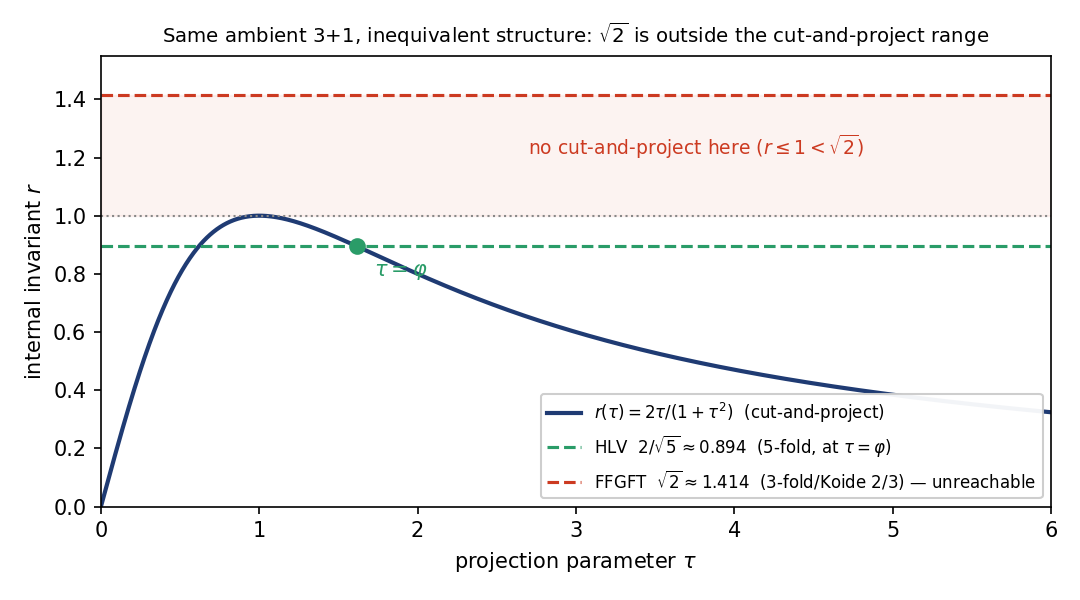
\includegraphics[width=0.92\linewidth]{../fig/fig_rtau_fork.png}
\caption{The cut-and-project invariant $r(\tau)\le 1$ reaches HLV's $2/\sqrt5$ at
$\tau=\varphi$ but never FFGFT's $\sqrt2$. That $\sqrt2$ lies above this family's maximum
means only that this particular projection does not interconvert the two invariants -- not
that the structures are incompatible (see next section).}
\end{figure}

\noindent What this shows -- and what it does not:
\begin{itemize}
\item \textbf{Ambient $3{+}1$:} both models end in $\mathbb{R}^3\times\mathbb{R}_t$; at the
level of the bare coordinate manifold this is a lossless representational transformation
(Type~III, Doc.~270/230).
\item \textbf{The cut-and-project map:} $\sqrt2$ lies outside the range $r\le1$, so
\emph{this} one-parameter family does not carry HLV's $2/\sqrt5$ into FFGFT's $\sqrt2$.
That is a statement about one map, \emph{not} a proof of incompatibility: reconciliation is
not ``interconvert the two invariants'' but ``embed both in a common structure'' -- the
subject of the next section. (And $\sqrt2>1$ versus $r\le1$ are not strictly commensurable,
so their non-equality here is weak evidence at best.)
\end{itemize}

% ==============================================================================
\section{The reconciliation: HLV contains FFGFT (\texttt{recompute\_reconcile})}
% ==============================================================================
The decisive fact is group-theoretic. The icosahedral group $A_5$ \emph{contains} the
$3$-fold $C_3$: a $120^\circ$ rotation about a $(1,1,1)$ axis and a $72^\circ$ rotation
about a vertex axis are \emph{both} symmetries of the same regular icosahedron -- both
permute its twelve vertices (\texttt{recompute\_reconcile.py}). Hence $C_3<A_5$, and at the
level of dimensions $T^7=T^4\times T^3$, i.e.
\begin{equation}
7 \;=\; \underbrace{3_{\text{phys}}+1_{\text{time}}}_{\text{FFGFT }T^4}\;+\;\underbrace{3_{\text{perp}}}_{\text{HLV extension}}.
\end{equation}
Concretely $T^4\hookrightarrow T^7$, $(x,t)\mapsto(x,0,t)$ with $0\in T^3_{\text{perp}}$ -- a totally geodesic submanifold: every FFGFT configuration is the special HLV configuration with vanishing perp coordinate. The relation between the models is therefore \emph{containment}, $\mathrm{HLV}\supset
\mathrm{FFGFT}$: FFGFT is the minimal crystallographic $3$-fold core, HLV the icosahedral
extension adding the three perp circles and the full $5$-fold. The protected values $\sqrt2$
and $2/\sqrt5$ are invariants of the coexisting $C_3$ and $A_5$ sectors of the \emph{same}
containing structure; they need not, and do not, transform into one another -- and that is
no contradiction. The containment is at the level of the groups and dimensions; the
\emph{protected} invariant remains a separate, realised choice -- FFGFT protects an
independent $3$-fold geometry ($\sqrt2$), HLV the $5$-fold ($2/\sqrt5$), and (Doc.~283)
HLV's protected vacuum directions do not include $\sqrt2$. Containment makes the models
compatible without making them identical.

\medskip\noindent\emph{Where this is asserted.} All of this lives in the compactified picture --- the tori with every circle compact, where no circle is singled out as time. The bridge to physical, decompactified observables runs through the single step $S^1\to\mathbb{R}$, the measurement (Doc.~270); the containment is therefore asserted upstream of the measurement, in the compact state, not on the physical-time axis.

% ==============================================================================
\section{Resolution}
% ==============================================================================
The tension -- ``both reduce to $3{+}1$, so the $3$ and the $6$ can only describe the same
thing'' -- is resolved not by a fork but by \emph{containment}. The $3$ and the $6$ share
the same physical $3{+}1$ core, and the models are mathematically reconcilable:
$\mathrm{HLV}\supset\mathrm{FFGFT}$ in both the symmetry ($A_5\supset C_3$) and the
dimensions ($7=4+3$). What remains is not a mathematical incompatibility but the question of
\emph{which symmetry sector is physically realised}. FFGFT realises the minimal,
crystallographic $3$-fold core, and its invariant -- Koide $\theta=2/9$ -- is empirically
confirmed; HLV adds the $5$-fold/perp structure as an extension whose distinct observable
(the icosahedral / quasicrystalline coherence signature, Doc.~282/283) is exactly what a
test of HLV against FFGFT would probe. The earlier wording is corrected in both directions:
``only a mathematical transformation'' is too weak (the realised sector is a genuine,
empirically decidable feature) and ``inequivalent, irreconcilable structures'' is too strong
(the embedding $\mathrm{HLV}\supset\mathrm{FFGFT}$ exists). The precise statement: a shared
$3{+}1$ core, with HLV the icosahedral \emph{extension} of FFGFT's minimal $3$-fold core,
the difference residing in the realised symmetry sector.

% ==============================================================================
\section{Recursion in the unified compact picture: $\lambda^n$}
% ==============================================================================
The notation $(T^N,G)$ extends to the \emph{recursion}: in both models the self-similar
structure is a dilation by a single eigenvalue $\lambda$, the recursion being $\lambda^n$.
The recursion eigenvalue is \emph{distinct} from the protected invariant ($\sqrt2$,
$2/\sqrt5$); conflating the two is an error.

\textbf{FFGFT: $\lambda=\xi=4/30000$ (Doc.~270).} The recursion $\xi^n$ is one-sided
contracting ($\xi,\xi^2,\dots$ vanish at once), giving the fractal correction
\begin{equation}
D_f = 3-\xi = 2.999867,
\end{equation}
a dimension just below $3$ -- near-crystalline. The protected invariant $\sqrt2$ (Koide
$2/3$) is a \emph{separate} quantity, not the recursion scale.

\textbf{HLV: $\lambda=\varphi$ (golden inflation).} The icosahedral quasicrystal is
self-similar under the golden inflation, with the Fibonacci recursion $\varphi^2=\varphi+1$.
The Fibonacci substitution matrix (rows $(1,1)$, $(1,0)$) has eigenvalues $\varphi$
(expanding) and $-1/\varphi$ (contracting) -- the \emph{same} $\varphi\leftrightarrow-1/\varphi$
pair as the $\mathbf 3\oplus\mathbf 3'$ physical/perp split. Being two-sided, the recursion is
self-similar at \emph{all} scales: a genuine quasicrystal. The protected invariant $2/\sqrt5$
is again separate.

\begin{center}\small
\renewcommand{\arraystretch}{1.2}
\begin{tabular}{@{}p{2.0cm} p{2.7cm} p{5.0cm} p{2.6cm}@{}}
\toprule
 & recursion $\lambda$ & character & protected inv. \\
\midrule
FFGFT & $\xi=4/30000$ & one-sided contracting, $D_f=3-\xi$ & $\sqrt2$ (Koide $2/3$) \\
HLV & $\varphi$ & two-sided ($\varphi,\,-1/\varphi$), $\varphi^2=\varphi+1$ & $2/\sqrt5$ \\
\bottomrule
\end{tabular}
\end{center}

\noindent So the fork appears once more, now in the recursion: $\xi$ tiny (one-sided,
near-crystalline) versus $\varphi$ golden (two-sided inflation). The extra contracting mode
($-1/\varphi$, the perp direction) is exactly HLV's extension over FFGFT, consistent with
$\mathrm{HLV}\supset\mathrm{FFGFT}$. In each model one number governs both the protected
geometry and the recursion.

A recursion \emph{phase} (an analogue of FFGFT's Koide angle $\theta=2/9$) is \emph{not}
fixed here. It would have to be \emph{derived} from the $A_5$ representation; the naive
$2/9+1/5=19/45$ is numerology, has no derivation, and is not adopted. Computed:
\texttt{recursion\_unify.py}.

\medskip\noindent\textbf{Status of $\varphi$.} The golden ratio acquires a meaning here that it lacked in pure FFGFT -- but \emph{not} as an FFGFT constant: as the derived eigenvalue of HLV's $5$-fold / perp sector, hence a marker of the boundary HLV$\setminus$FFGFT. This is consistent with Doc.~190 (P35): there $\varphi^N$ was the cautionary example of an arbitrary fitting base with no forward content; here $\varphi$ is the eigenvalue of a named symmetry (golden inflation $\varphi^2=\varphi+1$), not a measured scale forced into an exponent. So $\varphi$ does not become an FFGFT prediction.

% ==============================================================================
\section{The HLV phase from $A_5$: $\theta=0$, the amplitude carries the difference}
% ==============================================================================
The protected geometry can be sharpened to a \emph{phase}. FFGFT's Koide angle $\theta=2/9$
is a phase offset in the $3$-component circulant
\begin{equation}
\sqrt{m_k} = 1 + A\cos\!\left(\tfrac{2\pi k}{3}+\theta\right),\qquad k=0,1,2,
\end{equation}
whose Koide ratio is $Q=(2+A^2)/6$, \emph{independent of} $\theta$. The model content then
splits cleanly into amplitude $A$ and phase $\theta$.

\textbf{FFGFT.} $A=\sqrt2$ (the $3$-fold protected amplitude) and $\theta=2/9$ -- a
\emph{free}, empirical offset ($Q=2/3$ for any $\theta$; $2/9$ is the measured Koide phase),
giving $Q=2/3$.

\textbf{HLV.} $A=2/\sqrt5$ (the $5$-fold/icosahedral amplitude: the $5$-fold eigenvalue
phases $\mathrm e^{\pm2\pi i/5}$ fix it through the inner product $1/\sqrt5$). The protected
vacuum directions are symmetry-rigid, so there is \emph{no free offset}:
$\theta_{\mathrm{HLV}}=0$, giving $Q=(2+\tfrac45)/6=7/15$ -- exactly the value in the
Doc.~283 fork table.

So $A_5$'s eigenvalue phases play explicit, distinct roles: the $3$-fold phases $\pm2\pi/3$
set the circulant \emph{lattice} (both models); the $5$-fold phases $\pm2\pi/5$ (and
$\pm4\pi/5$ in $\mathbf 3'$) set HLV's \emph{amplitude} $2/\sqrt5$ -- not a free phase. The
honestly derived HLV phase is therefore $\theta_{\mathrm{HLV}}=0$, and the whole model
difference lives in the amplitude (protected invariant $\sqrt2$ vs $2/\sqrt5$, i.e.\ Koide
$2/3$ vs $7/15$).

\begin{center}\small
\renewcommand{\arraystretch}{1.2}
\begin{tabular}{@{}p{1.8cm} p{1.7cm} p{3.4cm} p{2.4cm} p{1.6cm}@{}}
\toprule
 & amplitude $A$ & phase $\theta$ & Koide $(2{+}A^2)/6$ & source \\
\midrule
FFGFT & $\sqrt2$ & $2/9$ (free, empirical) & $2/3$ & $3$-fold \\
HLV & $2/\sqrt5$ & $0$ (rigid, protected) & $7/15$ & $5$-fold \\
\bottomrule
\end{tabular}
\end{center}

\noindent This also disposes of the naive guess $\theta=2/9+1/5=19/45\approx0.422$: it
matches \emph{neither} the derived phase ($0$) \emph{nor} the Koide ratio
($7/15\approx0.467$), and is adopted nowhere. The result is derived under the $3$-component
Koide parametrisation; $\theta_{\mathrm{HLV}}=0$ follows from the rigidity of the
icosahedrally protected directions (cf.\ Doc.~283). Computed: \texttt{phase\_from\_a5.py}.

% ==============================================================================
\section{How FFGFT unrolls: decompactification as the bridge to observation}
% ==============================================================================
FFGFT unrolls by letting \textbf{one circle of the torus $T^4$ become time through the measurement
act} (type-I decompactification). The three remaining circles supply observed space but stay
structurally untouched. The recursion $\xi^n$ thereby becomes a continuous dilation flow with
log-period $|\ln\xi|=\ln 7500\approx 8.92$. Crucially, the unrolling is \emph{not} part of the
theory but the bridge to observation (Doc.~248, Doc.~270) --- the torus remains the original, the
unrolled space is the image.

\subsection{The compact form}
In the compact picture FFGFT is the four-torus $\mathcal{M}=T^4=(S^1)^4$ with $G=\mathbb{Z}_3$. All
four circles are \emph{equivalent} --- there is no distinguished time. The three space circles carry
the gauge structure (connection Laplacian); the fourth is the mass circle with the duality
$\tilde{T}\cdot m=1$.

\subsection{The measurement act unrolls one circle (type I)}
Decompactification is not a mathematical limit $S^1\to\mathbb{R}$ but a physical act: the measurement
selects one circle as time and unrolls it. This is a property of the \emph{embedded observer}
(Doc.~248), not of the geometry. The type-I map $S^1_{\text{mass}}\to\mathbb{R}_t$ turns the dual
mass $m=1/\tilde{T}$ into rest energy; in doing so the winding number is discarded --- the
information-discarding step that forces the observer into time.

\begin{center}
\begin{tabular}{@{}p{1.5cm} p{6.2cm} p{4.3cm}@{}}
\toprule
Type & What happens & Example \\
\midrule
I & one circle becomes time (unrolled, winding discarded) & $S^1_m\to\mathbb{R}_t$ \\
II & one circle stays compact (discrete spectrum) & $S^1_x\to S^1_x$ (unchanged) \\
III & lossless coordinate transformation & $T^4\to\mathbb{R}^3\times S^1$ \\
\bottomrule
\end{tabular}
\end{center}

Important for clean bookkeeping: \emph{observed} space $\mathbb{R}^3$ arises from the lossless
coordinate transformation (type III) $T^4\to\mathbb{R}^3\times S^1$ and carries continuous momenta;
the \emph{discrete, mass-bearing} spectrum, by contrast, sits on the compact $\mathbb{Z}_3$ fiber, not
on the unrolled axis. \enquote{Compact/discrete} (fiber, masses) and
\enquote{$\mathbb{R}^3$/continuous} (type-III projection, space) are thus two different things and
must not be conflated.

\subsection{The recursion unrolls along with it}
In the compact picture the recursion is discrete, $\lambda^n$ with $\lambda=\xi=4/30000=1/7500$. Upon
unrolling this becomes a continuous dilation flow $t\mapsto\xi t$, $t=t_0\,\xi^s$ ($s\in\mathbb{R}$)
--- the scale flow. A discrete scale invariance in the continuum is \textbf{log-periodicity} with
period $|\ln\xi|=\ln 7500\approx 8.92$ e-folds. This is a very long period; hence FFGFT is
\emph{near-crystalline}, the fractal correction tiny: $D_f=3-\xi=2.9998667$. The detailed treatment
(dilation flow, log-period, branching) follows in the next section.

\subsection{What survives --- and what does not}
\begin{center}
\begin{tabular}{@{}p{3.1cm} p{4.4cm} p{4.9cm}@{}}
\toprule
 & Compact ($T^4$) & Decompactified ($\mathbb{R}^3\times\mathbb{R}_t$) \\
\midrule
Mass circle & $S^1$, $m=1/\tilde{T}$ & $\mathbb{R}_t$, rest energy $E=m$ \\
Space & $3\times S^1$ & $\mathbb{R}^3$ (type III, continuous momenta) \\
Mass spectrum & eigenvalues of $S$ on the $\mathbb{Z}_3$ fiber (discrete) & unchanged; $m_k=\mu_k^2\,M$, $M=1/T$ \\
Recursion & $\xi^n$ (discrete) & $\xi^s$ (flow), log-period $\ln 7500$ \\
Symmetry & $\mathbb{Z}_3$ & $\mathbb{Z}_3$ (preserved) \\
Observer & none & embedded (measurement) \\
\bottomrule
\end{tabular}
\end{center}

The physics sits in the \emph{compact} picture and survives the unrolling because it consists of
\emph{ratios}: the $\mathbb{Z}_3$ symmetry (on the fiber, not on the torus), the Koide structure
($r=\sqrt2$, $\theta=2/9$, frame-independent), and the mass ratios. The mass operator
$S=\operatorname{circ}(t_0,t_1,t_2)$ does not change upon unrolling --- it lives on the $C_3$ fiber,
which is independent of the torus; the scale $M=1/T$ comes from the time circle. Only the winding
number of the unrolled circle is discarded. (Three time aspects: connection Laplacian without time,
process time via the non-Markovian kernel, geometry time via $\tilde{T}\cdot m=1$; Doc.~282.)

\emph{Consequence for the D7 comparison:} FFGFT unrolls the mass circle into time and keeps the
mass-bearing $3$-core; Kr\"uger's decompactified variant covers only $\{3'+\text{time}\}$ of this
(below). Computed: \texttt{decompact\_recursion.py}.

% ==============================================================================
\section{Decompactified recursive time: continuous dilation flow and log-periodicity}
% ==============================================================================
Compact and decompact are related by $S^1\to\mathbb{R}$ -- the measurement (Doc.~270), and
the recursion follows that map. In the compact picture the recursion is the \emph{discrete}
dilation $\lambda^n$ ($n\in\mathbb{Z}$): a \emph{discrete scale invariance} (invariance under
scaling by $\lambda$ only). When the mass circle unrolls to non-compact time, the discrete
recursion becomes a \emph{continuous} dilation flow
\begin{equation}
t\ \longmapsto\ \lambda\,t,\qquad t=t_0\,\lambda^{s},\quad s\in\mathbb{R},
\end{equation}
i.e.\ the renormalisation-group / scale flow. A discrete scale invariance in the continuum is
\emph{log-periodicity} of period $|\ln\lambda|$ -- equivalently, complex scaling exponents
$\alpha=\alpha_0+\mathrm i\,k\,2\pi/|\ln\lambda|$.

\begin{center}\small
\renewcommand{\arraystretch}{1.2}
\begin{tabular}{@{}p{1.8cm} p{2.6cm} p{6.2cm}@{}}
\toprule
 & compact & decompactified \\
\midrule
FFGFT & $\xi^n$ (discrete) & flow $t\to\xi t$; log-period $|\ln\xi|=\ln 7500\approx8.92$ \\
HLV & $\varphi^n$ (discrete) & flow $t\to\varphi t$; log-period $\ln\varphi\approx0.481$ \\
\bottomrule
\end{tabular}
\end{center}

\noindent The fork persists in decompactified time. \textbf{FFGFT}: a log-period of
$\approx8.9$ e-folds -- very long, so barely log-periodic; near-crystalline. It is the same
discrete scale invariance that gives $D_f=3-\xi$. \textbf{HLV}: a log-period of
$\approx0.48$ e-folds -- short and dense; a full quasicrystal, self-similar at every scale.

FFGFT's \emph{recursion $R$} is precisely this object: discrete ($\xi^n$) in the compact
picture, a continuous RG / scale flow once decompactified -- the $R$ reads both ways
(recursion $\leftrightarrow$ renormalisation flow). Computed: \texttt{decompact\_recursion.py}.

\subsection{Marcel's decompactified variant: the overdamped kernel is the decompactified empty window}
The doubling has two branches; decompactifying $S^1\to\mathbb{R}$ (the measurement) turns each
into a continuous scaling exponent $\alpha=\ln\mu$:
\begin{center}\small\renewcommand{\arraystretch}{1.15}
\begin{tabular}{@{}l r l@{}}
\toprule
branch & $\operatorname{Re}\alpha$ & decompactified character \\
\midrule
expanding $\varphi$ (the D4 core, masses) & $+0.481$ & relevant; coherence / revival (back-flow $5.125$) \\
contracting $-1/\varphi$ (the $3'$ window) & $-0.481$ & irrelevant; decaying / overdamped \\
\bottomrule
\end{tabular}
\end{center}
\noindent Both share $|\ln\varphi|\approx0.481$; only the sign differs. The decaying branch is
exactly HLV's overdamped, decaying kernel (Docs.~282--284): \textbf{Marcel's overdamped kernel is
the decompactified empty window} --- the compact \enquote{empty $3'$} ($\to0$ discretely) and the
decompactified \enquote{overdamped, decaying} ($\operatorname{Re}\alpha<0$, $\to0$ continuously)
are the same object on the two sides of the measurement.

Crucially, the containment survives decompactification. Decompactified D7 is \emph{not} the
overdamped kernel alone: it is the D4 core (the relevant, coherence-carrying $\varphi$-branch with
the masses and revival $5.125$) \emph{plus} the $3'$ window (the irrelevant overdamped branch).
The D4 core remains contained inside decompactified D7 as its relevant sector; Marcel's kernel is
the \emph{extra} window, not the whole. This is just the decompactified image of $T^4\subset T^7$.

Two caveats. The identification \enquote{overdamped kernel $=$ decompactified window} is a
proposed reading (both are the decaying, non-discriminating sector), not a theorem. And because
decompactification is the measurement (information-discarding), this branch sits on the
null-reproducible side by construction: the discriminating content (revival $5.125$) is in the
relevant D4 core, not in the overdamped kernel. Computed: \texttt{decompact\_branches.py}.

\subsection{Relation to Kr\"uger's HLV kernel and claim-state note}
Kr\"uger's actual HLV memory kernel is a positive mixture of decaying exponentials,
$K(t)=\sum_i w_i\,\tau_i^{-1}e^{-t/\tau_i}$ (Kr\"uger, \emph{Pre-Registered Null-Model Benchmark
for HLV-Constrained Memory Kernels}, 2026). Every mode is pure decay (scaling exponent
$\operatorname{Re}<0$), so the kernel \emph{is} the decompactified contracting $-1/\varphi$ window
of the previous subsection. Decisively, Kr\"uger's own pre-registered benchmark finds this kernel
statistically indistinguishable from a generic positive two-exponential kernel --- the uniqueness
gate stays false, \enquote{not a unique physical signature.} That is the null-reproducible side,
established by his result, not merely asserted by ours.

The full HLV operator adds a skew-adjoint phase channel ($J^\top=-J$) to the positive kernel. The
skew-adjoint (non-gradient) part is exactly the structure his claim-state note requires for
sustained recurrence --- pure gradient flow admits no cycles --- and it is the analogue of the
relevant, oscillatory FFGFT revival ($5.125$); the decaying kernel is the overdamped window. The
two sectors line up: discriminating content sits in the recurrent/coherent (non-gradient) part,
not in the decaying magnitude.

A third, sharper correspondence comes from the path-memory comparator (De~Jesus, HICE-MEM, for
Kr\"uger): temporal order is antisymmetric, $\mathrm{Area}(P)=\sum_{i<j}[A_i,A_j]$ with
$\mathrm{Area}(P^{\mathrm{rev}})=-\mathrm{Area}(P)$, so a single history's magnitude and spectrum
are \emph{even} under reversal --- the anti-Hermitian spectrum $\{i\lambda\}\mapsto\{-i\lambda\}$
is the same set. The order-sign is discarded unless contracted against an oriented reference (a
second history). This is the same structure as the measurement $S^1\to\mathbb{R}$ discarding
winding while the magnitude survives: the discriminating content is relational, not single-history.

Finally the claim-state. Kr\"uger's clarification note (2026) separates compact internal
Spiral-Time, SI measurement time, and the signal index $\Delta\Phi_{\mathrm{sig}}$, and forbids
their identification without an explicit projection/calibration map $K$ --- the same discipline as
\enquote{structure $\neq$ physics without a map.} No identification of the two spiral notions and
no holonomy is claimed here: Kr\"uger's Spiral-Time enters as a bounded kinetic prefactor
$A_\psi(t)$ on the kernel (benchmark) and as a triadic compact coordinate $\theta\in S^1$ (note),
neither of which is the log-periodic log-spiral of the decompactified recursion. Computed:
\texttt{marcel\_kernel\_match.py}.

\subsection{Kr\"uger's unrolled variant covers only $\{3'+\text{time}\}$ --- not the full D7}
A placement of the decompactified side, \emph{without} importing Kr\"uger's formulas. The compact
FFGFT result --- $6=3\oplus3'$ as a fractal internal recursion, purely from the golden ratio
(Fibonacci operator, eigenvalues $\varphi$ expanding / $-1/\varphi$ contracting) --- is derived and
script-covered (\texttt{recursion\_doubling\_empty.py}, \texttt{verify\_recursion\_doubling.py},
$11/11$) and stands independently of HLV. It is not touched here; the comparison below does not
bear on it.

Kr\"uger's latest decompactified construction (\emph{Recursive Spiral-Time Nesting as a Route to a
Six-Dimensional Host Carrier}, 2026, with the null-gated runs Zenodo 20770402\,/\,20772007) reaches
a $6$D host via a \emph{stability selection} (a spectral gap), \emph{not} via $\varphi$ --- a
different mechanism, no $\varphi$ substitute. What matters for compatibility, however, is not the
mechanism but \emph{what the unrolled variant fills}: exclusively the \textbf{empty} sector. Its
decaying kernel is the decompactified $-1/\varphi$ window (above); its host sector is candidate-only
and massless (\enquote{host dimension, not masses}); and its compact time satisfies
$\chi(t)\neq\ln t$ (clarification note), so it is not the log-spiral of the FFGFT recursion.

The full-text version (2026) adds the downstream chain BD3--BD5 (Zenodo 20773678): a native finite
carrier (BD3), a low-q Lorentz/EFT pre-screen (BD4) and semantic transfer (BD5). It only adds more
structure and still reaches no physics --- BD4-HARD itself flags the low-q behavior as
\emph{carrier-conditioned, not HLV-specific} (matched nulls also pass), and BD0/BD1 remain negative.
This reinforces the $\{3'+\text{time}\}$ picture: the carrier is more elaborate but massless
structure. (Kr\"uger dates the nesting idea itself to the January-2026 HLV foundation, Zenodo
18255159.)

In D7 bookkeeping --- $7=[\,3\text{-core (crystallographic, masses)}+\text{time}\,]+3'$ --- his
variant therefore unrolls only \textbf{$3'$ + time}: the empty perp window plus the unrolled time
axis ($S^1_m\to\mathbb{R}_t$, shared). The mass-bearing crystallographic $3$-core ($\varphi/\xi$,
$\sqrt2$, Koide $2/3$) is \emph{not reached} by it and remains FFGFT's. Strictly, his HLV ---
as decompactified-realized --- is \emph{not} the full D7 space, but the subsector
$\{3'+\text{time}\}$; the full D7 (mass core $+$ time $+\,3'$) is realized by FFGFT.

Hence compatibility, briefly: his side $\subseteq$ FFGFT's $\{3'+\text{time}\}$. The formal
containment $T^7\supset T^4$ ($A_5\supset C_3$) stands; it is only sharpened here as to \emph{where}
Kr\"uger's unrolled construction actually sits. This is compatible \emph{as long as he holds the
candidate-only line} (his gates B0--B7); were he later to overreach (\enquote{$6$D host $=$ physical
spacetime with masses}), compatibility would have to be re-examined --- at present he explicitly
does not. Covered by \texttt{decompact\_branches.py} and the emptiness theorem above; no new script
is needed for his formulas.

% ==============================================================================
\section{What the d7 sector computes: masses from $\xi$, spectra from $\varphi$}
% ==============================================================================
By analogy with $\xi$ one asks what the d7 model ($T^7$, $A_5$) computes. The honest answer is
\emph{not masses}. Masses are the output of the crystallographic $3$-fold sector with $\xi$,
which d7 already contains (HLV~$\supset$~FFGFT); d7 reproduces them \emph{through} its FFGFT
sub-part, not as new content. The \emph{extra} d7 structure ($5$-fold, perp directions,
$\varphi$) is exactly the part that does not carry masses. What it carries instead:

\begin{center}\small\renewcommand{\arraystretch}{1.2}
\begin{tabular}{@{}p{3.2cm} p{5.6cm} p{2.8cm}@{}}
\toprule
quantity & d7 / $5$-fold output & status \\
\midrule
protected amplitude & $2/\sqrt5$, Koide-analog $Q=7/15$ & derived number \\
phase & $\theta_{\mathrm{HLV}}=0$ (no free Koide angle) & derived \\
recursion scale & $\varphi$; tower $\varphi^n$; log-period $\ln\varphi\approx0.481$ & derived \\
spectrum & aperiodic quasicrystal gap spectrum, $\varphi$-scaling & discriminator (271/283) \\
\bottomrule
\end{tabular}
\end{center}

\subsection{Why the spectrum does not lead to masses here}
FFGFT's masses are themselves spectral -- eigenvalues of the $T^4$ connection-Laplacian, the
Koide circulant levels -- so the question is fair; the answer is about \emph{which} spectrum.
A mass is a sharp, isolated level, so reading masses off a spectrum requires a \emph{discrete
point spectrum}. The $3$-fold is lattice-compatible ($2\cos(2\pi/3)=-1\in\mathbb{Z}$): it
closes on a periodic torus into exactly three sharp eigenvalues $\{-1,-1,2\}$ -- the triple.
The $5$-fold is lattice-incompatible ($2\cos(2\pi/5)=1/\varphi\notin\mathbb{Z}$): no periodic
lattice carries it, so its only carrier is an aperiodic quasicrystal, whose spectrum is
\emph{singular-continuous} (Cantor-like) -- a dense set of gaps, self-similar under $\varphi$,
with no isolated levels (a Fibonacci chain fragments into gaps at every scale, against the few
bands of the periodic chain; \texttt{spectrum\_to\_mass.py}). There is no distinguished triple
to read masses off. Hence \enquote{spectrum~$\to$~mass} needs a point spectrum, i.e.\ a
periodic / crystallographic carrier -- and the only crystallographic part of d7 is its
$3$-fold core, i.e.\ FFGFT. The route always returns to FFGFT; the genuinely-d7 (aperiodic)
spectrum cannot deliver masses. And a dense self-similar spectrum has a level near \emph{any}
number, so $\varphi^N$ \enquote{fits} anything -- the P35 numerology trap (Doc.~190, R44): the
very richness of the quasicrystal spectrum is what makes reading a mass off it content-free,
whereas the sparseness of the discrete torus spectrum is what makes an eigenvalue there a
genuine prediction.

\subsection{Information content: structure spectrum vs energy spectrum}
The previous point must not be read as \enquote{the quasicrystal spectrum carries no
information.} It does -- a quasicrystal has \emph{two} spectra, differing in type. The
\emph{structure} (diffraction) spectrum $S(q)=|\sum_n e^{\mathrm i q x_n}|^2$ is \emph{pure
point}: sharp Bragg peaks at $\varphi$-module positions, here $\approx21\times$ above the noise
floor of a random null of identical composition (\texttt{quasicrystal\_information.py}). That
sharp, null-distinguishable order \emph{is} the information -- exactly HLV's
substrate-distinguishability claim, which stands. The \emph{energy} (Laplacian) spectrum is the
singular-continuous (Cantor) one of the previous subsection; it is what lacks sharp levels and
so yields no masses. The two are different objects: information lives in the relational
long-range order (structure spectrum), not in individual energy levels (the energy states are
critical / fractal, not clean nodes). The P35 caveat is therefore narrow: only fitting a
\emph{single target number} as $\varphi^N$ is content-free; the structural signature is not.

\noindent\emph{Residual, kept honest.} The place where the FFGFT analysis found an HLV
signature \emph{null-reproducible} is the \emph{temporal} over-damped memory kernel
(Doc.~282--284, biexponential, non-identifiable sector) -- the time domain, a different object
from the spatial structure spectrum. So: spatial structure informative (HLV's point holds);
temporal over-damped kernel = the standing critique. The discriminating content lives in the
structural / spectral signature (pure-point diffraction; periodic-vs-aperiodic peaks) -- the
discriminator of Doc.~271/272/283. FFGFT and HLV agree \emph{where} the information sits (in
the structure); the critique concerned a different (temporal) claim.

\subsection{The one place d7 could touch masses (conjecture)}
The $6=3\oplus3'$ split leaves the perp irrep $3'$ (character $1-\varphi=-1/\varphi$) as a
\emph{second} triplet position; FFGFT realises the one $3$ (charged leptons, Koide $2/3$), the
$3'$ is empty. \emph{If} a physical triple sat there, its prediction would be $Q=7/15$ -- a
falsifiable target, not a derived particle mass. Computed: \texttt{what\_d7\_computes.py}.

% ==============================================================================
\section{The electron mode in D7: the embedding exists, the mass-label is C$_3$-frame}
% ==============================================================================
A natural consistency question: if a mode is read off as the electron in D4, it must have an
image in D7, since $T^4\subset T^7$. It does. The electron mode lifts to the D7 mode with the
same winding on the four D4 circles and zero winding on the extra three; sitting entirely in
the D4 sub-block, its Laplacian eigenvalue --- the mass --- is unchanged. The translation is
the embedding itself.

This does not conflict with \enquote{masses require the D4 core.} The sharp label
\enquote{electron} is a C$_3$-protected (crystallographic) statement, not an $A_5$ one: the
electron mode is an eigenvector of the $3$-fold. The full D7 symmetry is $A_5$, whose $5$-fold
elements do not commute with C$_3$ --- they rotate the electron mode into a muon/tau mixture.
Under a genuine icosahedral $5$-fold rotation the electron direction keeps $0.762$ of its weight
and leaks $0.238$ into the $\mu/\tau$ directions (\texttt{electron\_mode\_in\_d7.py}). So in the
full $A_5$ frame \enquote{electron} is not a sharp eigenstate; to read it as the electron (a
sharp mass) one selects the C$_3$ eigenbasis --- the restriction to the crystallographic
sub-block, i.e.\ \enquote{going back to D4.} The correspondence is the embedding; the mass
read-out is the frame choice; the two are the same statement.

Two safeguards. The mixing is a change of basis, not a smearing: the $5$-fold rotates the
labelling frame and does not destroy the physical mode, which stays perfectly sharp in any
C$_3$ frame. And the mode stays in the periodic \enquote{$3$} block (point spectrum) --- it does
not leak into the aperiodic $3'$ sector; the $5$-fold only rotates $e\leftrightarrow\mu
\leftrightarrow\tau$ within the physical \enquote{$3$}. Finally, which frame counts as the
$3$-fold is, once again, the measurement (Doc.~270/248): the mode exists frame-independently in
D7, the sharp particle label is frame-dependent.

% ==============================================================================
\section{The 3$'$ is the first recursion: why recursion directions are empty in the compact picture}
% ==============================================================================
The split $6=3\oplus3'$ and the golden recursion are not two facts but one: the doubling
\emph{is} the recursion acting once. This section makes that explicit and draws the consequence
for the empty $3'$.

\subsection{The doubling is the recursion operator}
The Fibonacci / inflation operator is
\begin{equation}
M=\begin{pmatrix}1&1\\1&0\end{pmatrix},\qquad \det M=-1,\quad \operatorname{tr}M=1,\quad
\text{characteristic polynomial }\lambda^2-\lambda-1=0 .
\end{equation}
Its two eigenvalues are $\varphi=\tfrac{1+\sqrt5}{2}\approx1.618$ (expanding, $|\varphi|>1$) and
$-1/\varphi=\tfrac{1-\sqrt5}{2}\approx-0.618$ (contracting, $|{-}1/\varphi|<1$), and
$\varphi^2=\varphi+1$. Crucially, the Galois conjugate that distinguishes the two
$3$-dimensional $A_5$ irreps, $\varphi\leftrightarrow1-\varphi$, is exactly the contracting
eigenvalue: $1-\varphi=-1/\varphi$. So the two eigendirections of $M$ \emph{are} the two irreps:
\[
3 = \text{the }\varphi\text{ (expanding) eigenmode},\qquad
3' = \text{the }-1/\varphi\text{ (contracting) eigenmode}.
\]
The appearance of $3'$ alongside $3$ is therefore one application of the golden recursion --- the
doubling is the recursion's eigenstructure. (That $M$ is the recursion operator is confirmed by
$M^n=\bigl(\begin{smallmatrix}F_{n+1}&F_n\\F_n&F_{n-1}\end{smallmatrix}\bigr)$, the Fibonacci
numbers.)

\subsection{The internal branch is the window --- hence empty}
In the cut-and-project reading of a quasicrystal, physical space is the expanding direction
($\varphi$) and internal space is the contracting direction ($-1/\varphi$). Internal space
carries the acceptance \emph{window}, not physical positions. Under iteration the internal
component decays geometrically while the physical component grows:
\begin{center}\small
\begin{tabular}{@{}r r r@{}}
\toprule
$n$ & $|\text{physical }(\varphi)|$ & $|\text{internal }(3')|\sim(1/\varphi)^n$ \\
\midrule
0 & 1.01 & 0.27 \\
2 & 2.64 & 0.10 \\
8 & 47.4 & 0.0058 \\
20 & --- & $1.2\times10^{-9}$ \\
\bottomrule
\end{tabular}
\end{center}
\noindent The decay rate per step is $1/\varphi^2\approx0.382$. So the $3'$ (internal branch)
carries no physical positions and vanishes under the recursion: that is why it is empty.

\subsection{The general principle: the seed carries, the recursion is empty}
The crystallographic seed (the \enquote{$3$}, $\varphi$-branch) holds the masses; everything the
golden recursion generates from it --- the conjugate $3'$ and the $\varphi^n$ tower --- is empty
of \emph{new} mass content. \enquote{Empty} means no new sharp level / no new triple, not
\enquote{does nothing}: the recursion still carries structure (FFGFT's $\xi^n$ gives the fractal
correction $D_f=3-\xi$; HLV's $\varphi^n$ gives the quasicrystal window). Several earlier
results collapse into a single statement:
\begin{center}\emph{$3'$ empty $=$ recursion directions empty $=$ masses need the crystallographic
core $=$ the recursion sector has no point spectrum $=$ the cut-and-project internal space
carries no physical positions.}\end{center}

\subsection{Consequence for the 3$'$ candidate: why a dynamics is needed}
This gives a \emph{structural} reason for the gap noted earlier. Putting a physical triple into
the $3'$ means putting mass content into the internal / window space --- precisely what the
compact recursion keeps empty. It cannot be supplied by the recursion alone; it requires a
dynamics that fills the window (a Hamiltonian / interaction on the $7$D torus). So the
conditional $3'$ candidate (the neutrino sector) needs a dynamics not only for methodological
caution but for this structural reason: the recursion leaves that branch empty by construction.

\subsection{Check scripts}
\begin{itemize}
\item \texttt{recursion\_doubling\_empty.py} --- demonstration: $M$'s eigenstructure
($\varphi$ / $-1/\varphi$), physical vs internal under iteration.
\item \texttt{verify\_recursion\_doubling.py} --- assertions (PASS/FAIL): eigenvalues, char.\
poly, $1-\varphi=-1/\varphi$, $M^n$ Fibonacci, internal branch $\to0$ at rate $1/\varphi^2$.
$11/11$ PASS.
\end{itemize}

% ==============================================================================
\section{The recursion tower D(4+3n): height is empty, depth needs dynamics}
% ==============================================================================
From the previous section the doubling is one golden recursion. The construction iterates: each
recursion adds one $3$ (the contracting $-1/\varphi$ branch), giving a dimension tower
$D(4+3n)$, $n=0,1,2,\dots$
\begin{center}\small\renewcommand{\arraystretch}{1.15}
\begin{tabular}{@{}r l l@{}}
\toprule
$n$ & dim & \\
\midrule
0 & D4 & seed (FFGFT, crystallographic kernel) \\
1 & D7 & one recursion (the first $3'$) \\
2 & D10 & two recursions \\
3 & D13 & \\
100 & D304 & formally unbounded \\
\bottomrule
\end{tabular}
\end{center}
\noindent But the theorem of the previous section fixes what this means: each added $3$ is an
\emph{empty} internal window (the contracting $-1/\varphi$ branch, which $\to0$ under iteration).
Hence $100$ recursions are $100$ empty windows, \emph{not} $100$ physical layers; the masses
reside, at \emph{every} level of the tower, only in the D4 seed. The tower is a geometric
hierarchy (nested cut-and-project), not new testable content --- and the theorem is what keeps
it from becoming a number mill (one could otherwise assert arbitrarily many \enquote{levels},
all empty).

Two caveats. \textbf{(i)} \enquote{$+3$ per step} assumes every level repeats the icosahedral
$3+3$ pattern; a different non-crystallographic symmetry (e.g.\ $8$-fold, silver ratio
$1+\sqrt2$) would give a different increment, so $D(4+3n)$ is the icosahedrally-repeated choice,
not mandatory. \textbf{(ii)} Filling any window requires a dynamics --- the same open gap at
every level; the tower does not escape the gap, it multiplies it.

\medskip\noindent\textbf{Constructive consequence.} The productive next step is not height
(D10, D100 --- more empty windows) but depth: the dynamics that fills the \emph{first} window.
And one physically interesting first window already exists --- the $3'\to$ neutrino sector
(conditional, next section). That is where the lever is, not in counting up the tower. Computed:
\texttt{recursion\_tower.py}.

\subsection{Two recursions --- and what the empty windows are good for}
A natural tension: \enquote{each $+3$ step is one more recursion depth, recursions are fractal
deepenings --- but if they are all empty and 4D already carries everything, why should unrolling
yield mass?} It resolves once two \emph{distinct} recursions, easily conflated, are separated:
\begin{itemize}
  \item \textbf{Scale recursion} $\xi_{n+1}=\xi_n(1-100\xi)$: refines the \emph{same} four
  dimensions across scales (log-period $\ln 7500$) and carries $D_f=3-\xi$ resp.\ $K_{\text{frak}}$
  --- it adds \emph{no} dimension. This is the actual \enquote{fractal deepening}.
  \item \textbf{Dimensional recursion} $D(4+3n)$ (golden operator, $\varphi$/$-1/\varphi$): stacks
  empty $3'$/$3''$ windows; the inner-branch weight decays $(1/\varphi^2)^n\to0$, no point spectrum.
\end{itemize}
The mass content upon decompactification comes from unrolling the \emph{mass circle} (4th circle of
D4, $\tilde T\cdot m=1$, type~I), which supplies the \emph{single} scale $M=1/T$; the dimensionless
ratios were already present compactly in 4D. The Kaluza-Klein intuition (unroll an extra dimension
$\to$ mass tower) thus applies to the mass circle, \emph{not} to the $3'$/$3''$ windows: an empty
window unrolled yields empty perp space, no mass tower, as long as no \emph{dynamics} (a Hamiltonian
on the window) fills it.

What, then, is the recursion good for if it yields no new masses? Not for levels, but for
\emph{structure}: the scale recursion carries the fractal correction ($D_f$, $K_{\text{frak}}$), the
dimensional recursion carries the cut-and-project \emph{window} that shapes the aperiodic order and
the \emph{spectral fine structure} (splitting, inharmonicities) on top of the crystallographic base
levels --- not new fundamental tones but their fine structure. The $3'$ window is in this sense a
\emph{slot} provided by the geometry; whether it gains physical content is decided by a dynamics
(the conditional neutrino candidate, next section), not by mere unrolling. Computed:
\texttt{klaer\_rekursion\_masse.py}.

% ==============================================================================
\section{Candidate for the 3$'$: the neutrino sector (conditional)}
% ==============================================================================
What could sit in the empty 3$'$? An \emph{open} question --- a conditional target, not a
prediction. The discriminator is the Koide ratio $Q=\sum m/(\sum\sqrt m)^2$; the conditional
3$'$ target would be $Q=7/15\approx0.467$. The measured triples:

\begin{center}\small\renewcommand{\arraystretch}{1.2}
\begin{tabular}{@{}p{5.6cm} p{2.6cm} p{3.4cm}@{}}
\toprule
triple & $Q$ & \\
\midrule
charged leptons $e,\mu,\tau$ (the \enquote{$3$}) & $0.667$ ($=2/3$) & far above target \\
up quarks $u,c,t$ & $0.849$ & far above target \\
down quarks $d,s,b$ & $0.731$ & far above target \\
\bottomrule
\end{tabular}
\end{center}

\noindent All measured charged triples have $Q\ge0.67$ --- none matches $7/15$; they are
excluded as a $7/15$ carrier (robust, also under the mass uncertainties). One open candidate
remains: the \textbf{neutrinos}. Their $Q$ is not fixed, because the absolute mass scale is
unknown; in a scan (normal ordering) $Q\approx0.586$ for a hierarchical spectrum and falls
towards $1/3$ as the scale grows. It crosses $7/15$ at a lightest mass $m_0\approx1.9$~meV
($\sum m_\nu\approx61$~meV, within the cosmological bound $\sim120$~meV). Structurally this is
the natural partner: leptons split into a charged triple (the \enquote{$3$}) and a neutral one
(neutrinos), and the second $3$ irrep is the slot for the neutral triple.

\medskip\noindent\textbf{Status (strict).} This is a conditional target, \emph{not} a
prediction. $Q$ varies \emph{continuously} with $m_0$, so \enquote{$7/15$ is hit} carries
content only if $7/15$ is fixed independently by a dynamics (the missing piece from the section
\enquote{Status of the D7 mass calculation}) \emph{and} beats a null. It is exactly Marcel
Kr\"uger's structure: carrier $=$ neutrinos, observable $=$ Koide $Q$, null control $=$ against
generic triples. That lifts the question from \enquote{guessing} to a \enquote{pre-registrable
target} --- no more. Computed: \texttt{which\_triple\_in\_3prime.py}.


\paragraph{Interpretation (conjecture, not derived from the theorems).} That the recursion
sector carries no point spectrum is consistent with the peculiar character of the neutrino
sector. It yields, however, no masses, no $\Delta m^2$ and no mixing angles --- these require the
still-missing dynamics. And the tower adds empty windows, not additional neutrino species.

\paragraph{Which energy type fills the window --- and the open computational gap.} Through
$\tilde T\cdot m=1$ FFGFT enforces \emph{two} energy types (Doc.~255): \emph{static} (rest mass $=$
topologically frozen winding, the crystallographic core) and \emph{kinetic} (free; for massless
states the only form, $E=hf$) --- \enquote{mass is frozen kinetic energy}. The dynamics that fills
the $3'$ window --- the temporal, holographic scale evolution (Doc.~263) --- therefore supplies the
\emph{kinetic} type, not frozen rest mass: a filled window is photon-/neutrino-like (massless /
near-massless), not a massive triple. This matches the neutrino as a \enquote{near-massless photon}
(Doc.~047, $m_\nu\sim\tfrac{\xi^2}{2}m_e$) and time-as-energy $\tilde T=1/\max(m,\omega)$
(Doc.~067/080): for $m=0$, $\tilde T=1/\omega$.

\emph{Open computational gap.} What is missing is the \emph{derived} rule to compute the kinetic
part, via the duality, as a \emph{$\xi$-fractal} fraction of the static part. The framework exists
(Doc.~080: $\tilde T=1/\max(E,\omega)$, electron $=$ rest $+$ $\gamma$-kinetic, photon $=$ purely
kinetic) and \emph{one} instance exists (Doc.~047: $\xi^2/2$ suppression --- but as an ansatz, not
derived; Doc.~204 has a $\xi$ correction to the kinetic energy). The general derivation
\enquote{kinetic $=$ $\xi$-fractal fraction of the static, via $\tilde T\cdot m=1$} is precisely the
still-missing dynamics --- the next computational step, not a solved piece.

% ==============================================================================
\section{Status of the D7 mass calculation: the gap and the next step}
% ==============================================================================
The HLV construction provides a consistent geometric embedding ($T^7$, $A_5$, $3\oplus3'$) and
qualitative predictions ($5$-fold coherence, $2/\sqrt5$ rather than $\sqrt2$). An explicit mass
formula on $T^7$ does not exist, however --- symmetry alone does not fix the mass matrix. What
is missing is a specified dynamics (Hamiltonian, interactions) on the 7D torus. Until that is
given, the $5$-fold predictions stay qualitative (\enquote{there should be signatures}) rather
than quantitative (\enquote{at this value}). FFGFT therefore remains the only model with an
explicit, tested mass formula. HLV is a structural conjecture that needs a dynamics --- and that
is the next construction site.

% ==============================================================================
\section{Where the fractal corrections sit}
% ==============================================================================
The fractal corrections sit at two causally chained levels --- and explicitly \emph{not} in the
ratios.

\subsection{Root: the conformal fractal metric}
The fundamental fractal quantity is $\xi=4/30000$ with the recursion
$\xi_{n+1}=\xi_n(1-100\xi_n)$ (Doc.~133/275). Its metric manifestation is \emph{conformal}, not
diagonal:
\[
g_{\mu\nu}^{\text{(frac)}}(x)=\eta_{\mu\nu}\,(1+\xi\,f(x)),\qquad D_f=3-\xi\quad(\text{Doc.~051}),
\]
with the $\xi$ correction specifically on the time component, $ds^2=(1+\xi\lambda_0/E_\xi)\,dt^2-dx^2$
(Doc.~025). In the winding/harmonic structure it appears as the damping exponent $\tau^{-(1+\xi)}$
(Doc.~159). \emph{Not} as a static metric $\mathrm{diag}(1,1,1,1+\xi)$ --- this form is unsupported;
the mass circle is distinguished via $\tilde{T}\cdot m=1$.

\subsection{Level~1: local spacetime porosity}
The first manifest correction is the local spacetime dimension
\[
D_f^{\text{space}}=3-\xi\approx 2.99987\quad(\text{Doc.~133}),
\]
a tiny deviation from integrality ($\sim0.003\%$, effectively~$3$). This is \emph{not} the type-II
projection (Doc.~270: $T^4\to T^3\to\mathbb{R}^3$, clean, for large $R$); the porosity is a separate
quantum-gravitational effect.

\subsection{Level~2: effective dimension and $K_{\text{frak}}$}
Through the cumulative RG run (17 orders of magnitude, Planck $\to$ electroweak) the porosity becomes
an \emph{effective} dimension $D_f^{\text{eff}}\approx2.973$, which Doc.~133 states is \enquote{not
identical} to $D_f^{\text{space}}$. From it the correction for absolute values emerges:
\[
K_{\text{frak}}=\left(\frac{D_f^{\text{eff}}}{3}\right)^{\!D_f^{\text{eff}}/2}\approx 0.9867
\approx 1-100\xi .
\]
The causal chain:
\[
\underbrace{3-\xi}_{\text{porosity}\ \sim0.003\%}\ \xrightarrow{\ \text{RG run, 17 OoM}\ }\
\underbrace{D_f^{\text{eff}}\approx2.973}_{\text{effective}}\ \xrightarrow{\ \text{formula}\ }\
\underbrace{K_{\text{frak}}\approx0.9867}_{\sim1.3\%}.
\]
$K_{\text{frak}}$ is thus \emph{not} an independent correction \enquote{at the SI step} but the
RG-cumulated consequence of $3-\xi$; it becomes visible only in the absolute/SI transition
(Doc.~122).

\subsection{Where they do \emph{not} sit}
\begin{center}
\begin{tabular}{@{}p{5.2cm} p{6cm}@{}}
\toprule
Quantity & contains $\xi$ / $K_{\text{frak}}$? \\
\midrule
$r=\sqrt2$, $\theta=2/9$ & no (pure $\mathbb{Z}_3$ structure) \\
$\mu_k$ (eigenvalues of $S$) & no \\
mass ratios, $\alpha$ as ratio & no ($K_{\text{frak}}$ cancels) \\
Koide $Q=2/3$ & no (pure $\mathbb{Z}_3$ structure) \\
$D_f^{\text{space}}=3-\xi$, $D_f^{\text{eff}}$ & yes (dimension) \\
absolute values ($m$ in kg, $G$ in SI) & yes ($K_{\text{frak}}$) \\
\bottomrule
\end{tabular}
\end{center}
The corrections affect only the dimensions ($D_f^{\text{space}}$, $D_f^{\text{eff}}$) and the absolute
values ($K_{\text{frak}}$). \textbf{Ratios are $\xi$- and $K_{\text{frak}}$-free} --- the decisive
statement from Doc.~101/122.

% ==============================================================================
\section{From geometry to SI: the conversion}
% ==============================================================================
This closing bridge is \emph{purely conventional} --- it adds no physics but translates the geometric
quantities into human-made units. The only fundamental object is the dimensionless number
$\xi=4/30000$; $c,\hbar$ are conventions (SI-2019), $G$ is measurement data, and mass ratios, Koide
$2/3$ and $\alpha$ are dimensionless ratios (Doc.~101, Doc.~122). The decisive separation:
\emph{ratios} are unit- and $K_{\text{frak}}$-free; the fractal correction
$K_{\text{frak}}=1-100\xi\approx 0.9867$ appears \emph{only} in the step from ratio to
\emph{absolute} (SI) value. The \enquote{circularity} of the conversion is thus metrological
(SI-2019), not a physical problem (Doc.~101).

\subsection{The compact quantities (purely geometric)}
\begin{center}
\begin{tabular}{@{}p{1.7cm} p{3.4cm} p{6.4cm}@{}}
\toprule
Quantity & Compact value & Meaning \\
\midrule
$r$ & $\sqrt2$ & $\mathbb{Z}_3$ circulant amplitude \\
$\theta$ & $2/9$ & $\mathbb{Z}_3$ phase \\
$\xi$ & $4/30000$ & fractal recursion (fundamental) \\
$\mu_k$ & $\{0.04035,\ 0.58021,\ 2.37944\}$ & dimensionless eigenvalues of $S$ \\
$Q$ & $2/3$ & Koide invariant \\
\bottomrule
\end{tabular}
\end{center}
These are unit-free and $K_{\text{frak}}$-free.

\subsection{The scale $M$ from the time circle}
The mass circle $S^1$ carries, via $\tilde{T}\cdot m=1$, the \emph{only} dimensionful quantity
$M=1/T$ --- a mass in natural units. It is fixed from \emph{one} measured mass (the muon):
\[
M=\frac{m_\mu^{\text{meas}}}{\mu_\mu^2}=\frac{105.6583755}{0.58021^2}\approx 313.86\ \text{MeV}.
\]
All other masses are then \emph{predicted} --- that is the test of the theory.

\subsection{The masses (ratio level, $K_{\text{frak}}$-free)}
\begin{center}
\begin{tabular}{@{}p{2.2cm} p{1.9cm} p{3.4cm} p{3.4cm}@{}}
\toprule
Lepton & $\mu_k$ & $m_k=\mu_k^2 M$ (MeV) & measured (MeV) \\
\midrule
Electron & $0.04035$ & $0.51100$ & $0.51099895$ \\
Muon & $0.58021$ & $105.658$ (anchor) & $105.6583755$ \\
Tau & $2.37944$ & $1776.98$ & $1776.86$ \\
\bottomrule
\end{tabular}
\end{center}
The mass ratios are unit- and $K_{\text{frak}}$-free: $m_\mu/m_e=206.77$, $Q=2/3$. (Electron to five
figures, tau as a $\sim0.007\%$ prediction; the $\mu_k$ follow from $r=\sqrt2$, $\theta=2/9$, fixed by
Koide $+$ (e,$\mu$).)

\subsection{The fine-structure constant $\alpha$ (ratio level)}
\[
\alpha=\xi\left(\frac{\sqrt{m_e\,m_\mu}}{\text{MeV}}\right)^2 .
\]
With $\sqrt{m_e\,m_\mu}\approx 7.348$ MeV: $\alpha\approx 0.007199$, i.e.\ $1/\alpha\approx 138.9$; the
exact bridge value $E_0=7.398$ MeV gives $1/\alpha=137.04$ (the $\sim1.3\%$ is the radiative-correction
level). $\alpha$ too is unit- and $K_{\text{frak}}$-free; $E_0$ is a bridge constant from the mass
ratios (Doc.~101).

\subsection{The gravitational constant $G$ (absolute level, with $K_{\text{frak}}$)}
$G$ is the only quantity that needs a genuine SI conversion
($[G]=\text{m}^3\,\text{kg}^{-1}\,\text{s}^{-2}$). The structural derivation (Doc.~006/122/133) yields
it as an absolute value in which the fractal correction appears \emph{only here}:
\[
G_{\text{SI}}=\frac{\xi^2}{4M}\cdot\frac{\hbar c}{(1\,\text{MeV})^2}\cdot K_{\text{frak}},
\qquad K_{\text{frak}}=1-100\xi=0.9867,
\]
\[
G_{\text{SI}}\approx 6.674\times10^{-11}\ \text{m}^3\,\text{kg}^{-1}\,\text{s}^{-2}.
\]
This is the \emph{computed} gravitational constant (not an input); the scale anchoring via the RG
amplification is given in Doc.~133/275, not in this conversion.

\subsection{The general conversion rule}
\[
\boxed{\ \text{quantity}_{\text{SI}}=\text{quantity}_{\text{geom}}\times\text{conversion factors}\times K_{\text{frak}}\ }
\]
with the conversion factors $\hbar,c$ and the scale $M$ (convention, SI-2019). The separation in one
line:
\begin{center}
\begin{tabular}{@{}p{3cm} p{6.2cm} p{2.8cm}@{}}
\toprule
Level & Quantities & $K_{\text{frak}}$ \\
\midrule
Ratio & $m_\mu/m_e$, $m_\tau/m_\mu$, $Q$, $\alpha$ & cancels out \\
Absolute (SI) & $m_e,m_\mu,m_\tau,G$ & appears \\
\bottomrule
\end{tabular}
\end{center}
References: Doc.~101 (circularity is metrological), Doc.~122 (ratio vs absolute, $K_{\text{frak}}$),
Doc.~133/006 (derivation of $G$ with $E_0$, $K_{\text{frak}}$, scale).

% ==============================================================================
\section{BD12-XCORE: the FFGFT mass-core declaration}
% ==============================================================================
Kr\"uger's open question --- what makes a \emph{legitimate} mass-core docking criterion rather than a
post-hoc fit --- FFGFT answers operationally, not by assertion: with a \emph{frozen, pre-registered}
declaration in matched-null format (his BD style). The rule has \emph{no} free parameters: $r=\sqrt2$,
$\theta=2/9$, and the Z$_3$/Foot-Koide spectrum $\mu_k = 1+\sqrt2\cos(\theta+2\pi k/3)$.

It produces: Koide $Q=\Sigma\mu^2/(\Sigma\mu)^2 = 2/3$ exactly (forced by $r=\sqrt2$); the lepton
ratios $m_\mu/m_e$ to $0.001\%$, $m_\tau/m_e$ to $0.007\%$; and --- as a \emph{genuine prediction}
from Koide $+\{m_e,m_\mu\}$, with no $\tau$ input --- $m_\tau=1776.97$~MeV against $1776.86$ measured
($0.006\%$). The matched-null test (tolerance Koide $0.1\%$, ratio $1\%$) shows: random $r$ hits Koide
in $0.18\%$, random $\theta$ both ratios in $0.025\%$, random $(r,\theta)$ the \emph{joint} set in
$0.000\%$ of cases. The frozen rule is therefore \emph{special}, not a generic fit ---
\textbf{PASS}; and symmetric, random inputs would give \textbf{FAIL}.

Two constraints keep the dock honest: (i) do \emph{not} dock on $L_{\text{nat}}$ --- the masses are not
in the carrier Laplacian but in the compact Z$_3$ core $+$ mass-circle ($\tilde T\cdot m=1$); (ii) the
dock is a \emph{fixed transformation} (a pre-registered algebraic map onto $\{\sqrt2,\,2/9,\,M=1/T\}$),
adding no new physics --- hence \emph{not} a post-hoc fit, but an equivalence that reproduces or
fails. Computed: \texttt{bd12\_xcore\_ffgft.py}.

% ==============================================================================
\section{Reproducibility}\label{sec:repro}
% ==============================================================================
\begin{itemize}
\item \texttt{dim\_bridge\_1\_doubling.py} -- $\mathbf 6=\mathbf 3\oplus\mathbf 3'$;
characters $\varphi$, $1-\varphi$, integer $6$D character; orthogonality and order $5$.
\item \texttt{dim\_bridge\_2\_crystallographic.py} -- crystallographic restriction
$2\cos(2\pi/n)$; $3$-fold integer, $5$-fold $=1/\varphi$.
\item \texttt{dim\_bridge\_3\_same\_ambient\_fork.py} -- $r(\tau)\le1$; $2/\sqrt5$ at
$\tau=\varphi$; $\sqrt2$ above the family's maximum (a statement about one map only).
\item \texttt{recompute\_reconcile.py} -- $C_3<A_5$ ($3$-fold and $5$-fold both permute the
same icosahedron) and $7=4+3$; the containment $\mathrm{HLV}\supset\mathrm{FFGFT}$.
\item \texttt{recursion\_unify.py} -- recursion $\lambda^n$: $\lambda=\xi$ ($D_f=3-\xi$) vs $\lambda=\varphi$ ($\varphi^2=\varphi+1$).
\item \texttt{phase\_from\_a5.py} -- the $A_5$ phase: $\theta_{\mathrm{HLV}}=0$, $Q=7/15$; $19/45$ excluded.
\item \texttt{decompact\_recursion.py} -- decompactified recursion: discrete $\lambda^n\to$ continuous flow $t\to\lambda t$, log-period $|\ln\lambda|$.
\item \texttt{what\_d7\_computes.py}, \texttt{spectrum\_to\_mass.py} -- what the d7 sector computes (no masses; $Q=7/15$, $\varphi$, spectra) and why a point spectrum is needed for masses.
\item \texttt{quasicrystal\_information.py} -- structure (diffraction) spectrum pure-point vs random null: the substrate's information content.
\item \texttt{electron\_mode\_in\_d7.py} -- the electron mode embeds in D7 (T$^4\subset$T$^7$); a 5-fold rotates it (0.762/0.238), so the sharp mass-label is C$_3$-frame = the D4 core.
\item \texttt{which\_triple\_in\_3prime.py} -- candidate triples for the 3$'$ via Koide $Q$: leptons/up/down excluded ($Q\ge0.67$), neutrinos the open candidate (crosses $7/15$ at $m_0\approx1.9$~meV).
\item \texttt{recursion\_doubling\_empty.py}, \texttt{verify\_recursion\_doubling.py} -- the 3$'$ as the contracting ($-1/\varphi$) recursion eigenmode; internal branch $\to0$ (11/11 PASS).
\item \texttt{recursion\_tower.py} -- the tower $D(4+3n)$ (D4/D7/D10/\dots/D304) and the emptiness of every added window.
\item \texttt{decompact\_branches.py} -- the two branches decompactified ($\operatorname{Re}\alpha=\pm0.481$): $\varphi$ relevant (D4 core), $-1/\varphi$ overdamped (Marcel's kernel); D4 core stays contained.
\item \texttt{marcel\_kernel\_match.py} -- grounded match to Kr\"uger's kernel $K(t)=\sum_i w_i\tau_i^{-1}e^{-t/\tau_i}$ (overdamped $=$ $-1/\varphi$ window) and the antisymmetric path-memory order (single-history spectrum even under reversal).
  \item \texttt{bd12\_xcore\_ffgft.py} -- the BD12-XCORE declaration: frozen rule ($r=\sqrt2$, $\theta=2/9$), Koide $2/3$, ratios, $\tau$-prediction and the matched-null test (nulls $0.000\%$ on the joint set).
\end{itemize}
All scripts are \texttt{numpy}-only with fixed values. Note: the $\sqrt2$ appearing at
$n=8$ in the crystallographic table is $2\cos45^\circ$ (the octagonal rotation), a
numerical coincidence -- not FFGFT's $\sqrt2$, which is the Koide/$\mathbb{Z}_3$-circulant
ratio \emph{within} the crystallographic $3$-fold structure, not a rotation order.
